%!TEX root = ../template.tex
%%%%%%%%%%%%%%%%%%%%%%%%%%%%%%%%%%%%%%%%%%%%%%%%%%%%%%%%%%%%%%%%%%%%
%% chapter2.tex
%% NOVA thesis document file
%%
%% Chapter with the template manual
%%%%%%%%%%%%%%%%%%%%%%%%%%%%%%%%%%%%%%%%%%%%%%%%%%%%%%%%%%%%%%%%%%%%
\chapter{Related Work}
\label{cha:users_manual}

% ================
% = Introduction =
% ================
In this chapter we address existing solutions that are able to protect applications from the OS or hypervisor, regardless the machine where they're running on (whether running locally or in cloud), thus increasing the level of trust an user can deposit in an execution of an application.

These existing solutions are organized in different sections in the following way: Section 2.1 covers Trusted Computing Environments; Section 2.2 covers software approaches that enable protection against untrusted OSes by making use of Trusted Execution Environments; Section 2.3 covers Intel-SGX frameworks; 

Finally, in Section 2.4 we make a critical analysis on the previously discussed techniques, while covering it's main advantages and disadvantages.


\section{Trusted Computing Environments} % (fold)
\label{sec:introduction}
We're currently in a period where we start to depend more and more on allowing other services to do our work for us. Technologies like cloud computing require users to trust these systems. Therefore it's needed something to grant some respectable level of security, as well as being able to grant trust to the user. That's were Trusted Computing Environments (TCE) come in handy.
A TCE is a concept that came to grant integrity and confidentiality to systems by forcing a certain machine to behave an expected way, and deny any unwanted access to the data while decrypted. This way, even if the system does not run in a trusted machine, it can be expected that it will execute as it should. 

TCEs protect the system against components that should always be trusted, like the host OS or even system admins, due to the priviledges they've got. Thus preventing this components from abusing these privileges, and always guarantee the normal execution of the system. 

In the following sections, as said before, we'll see how to achieve this properties, what components can be used to do it and also how each one of them works.

\subsection{TPM – Trusted Platform Modules }

A Trusted Platform Module (TPM), proposed by the Trusted Computing Group (TCG), is a set of hardware and software technologies that aim to create trust in a local platform \cite{sgxCloudThesis}. It is identified by an Endorsment Key-pair (EK) which is unique for every TPM, and also a Storage Root Key (SRK) that is used to protect other keys and data in the TPM. 

As for the hardware, a TPM consists mainly on a chip, found usually in the motherboard of most machines nowadays, that provides and stores cryptographic keys that can be used to grant integrity and data confidentiality to the system, as well as persistent and volatile memory to store these keys. 

As said before, the main objective of a TPM is to create the idea of a trusted platform. This will be  provided by three main services: Encryption, Authenticated Boot and Attestation. The first one is used for pretty much every aspect related with security and privacy. The Authenticated boot consists in booting the OS in stages, as a way of keeping track of which code is trustable through the usage of Platform Configuration Registers (PCR), that store the trusted software hashes. As for the Attestation, we'll see in the next subsection.


\subsection{TPM – Enabled Software Attestation}


TPMs enable the use of Remote attestation, which is the capability of one system to determine if other system can be trusted to run a particular piece of software as expected or not.

This is made possible by having a trusted configuration of state as reference, provided by the PCRs defined in the boot sequence, followed by a remote system that proceeds to challenge the trusted platform (containing the TPM) with a nonce. Then the platform creates a message with the nonce received previously and the existing configuration and calculates an hash value for that message. With an Attestation Identity Key (AIK), the message is then signed and sent back to the remote system, which then proceeds to decrypt the message with the EK public part, that then compares the result with the hash of the nonce plus the configuration it had at the begining of the challenge. 

If the hashes match, the remote system can then identify the TPM platform as a trusted platform.

\subsection{HSM – Hardware Security Modules}

Hardware Security Modules (HSM) are physical components whose main function is to provide and store cryptographic keys used to encrypt/decrypt data inside a system. HSMs can also perform cryptographic operations (e.g. encryption, hashing, etc.) as well as authenticate through verification of digital signatures and accelerate SSL connections \cite{hsmThesis}.

This modules are used mainly in large environment systems (e.g. large distributed systems) where there are a lot of machines communicating with each other, therefore creating a more needed sense of security. The inclusion of this modules in these big systems is actually a good idea since HSMs can also help servers relieve the workload coming from cryptographic operations. However HSMs don't quite guarantee the idea of absolute security, but increment the cost of attacking the system.

Although HSMs grant some extra level of security to a system, there's some drawbacks. One of them is the cost, where to buy one HSM the price varies depending on the sophistication of the security, plus the cost of maintenance makes it even more expensive. Another disadvantage is the difficulty on updating the module. Let's say a weakness was found in a cryptographic algorithm, it's hard to update the software in an already functional HSM to eliminate that weakness \cite{hsmPaper}.

\subsection{Trusted Execution Environments}

A Trusted Execution Environment (TEE) is an abstraction provided by both software and hardware that guarantees isolated execution of specific programs from other programs running on the same machine \cite{guiBorgesThesis}, but also from the host OS, hypervisor or even system administrators, preventing them from leveraging their priviledges and thus take advantage of the system. A TEE also grants secured storage of sensitive data, as well as remote attestation to make sure a given program runs as expected on a remote TEE. 

For a user to communicate with his program running inside an isolated environment, a key-exchange between the TEE and the user takes place. This way it is ensured both integrity and confidentiality of data during further communications.

This TEE abstraction can be achieved either by using a virtual machine monitor or by running security critical software (from whole applications to little segments of code) under protection mechanisms provided by hardware \cite{pcopThesis}. 

In the next chapters we will be looking into more dept about this hardware protection providers, that are responsable to create this trusted environments in the systems nowadays.

\subsection{Intel SGX}

Intel Security Guard Extensions (SGX) are a set of instructions built in Intel CPUs, that allow programmers to create TEEs, called enclaves. Enclaves are isolation containers that create an isolated environment where sensitive code can be stored and executed inside, ensuring integrity and confidentiality to it. By doing so, it reduces the Trust Computing Base, in a way that most of the system software, apart from the enclaves itself, is considered not trusted.

Enclaves are mapped into private regions of memory, where only the CPU as access to, reducing the TCB to only the enclave and the CPU itself. Due to this restrictions, not even the most common system libraries can be accessed inside the enclave, since the OS is not trusted. 

A system that encorporates the SGX under it's architecture is divided in two components, a trusted being the enclave, and an untrusted being the rest of the system. The untrusted component requests the launch of the enclave, where the CPU then manages to allocate the enclave in a private region of memory, made available only to that particular enclave. This portion of memory is kept encrypted in volatile memory, being only decrypted by the CPU if the responsible enclave requests for it \cite{guiBorgesThesis}.

Altough isolation is the main objective of Intel SGX, it still allows a way for both  untrusted and trusted parties to communicate. This is made possible by the functions ECALL and OCALL. ECALLs are used for an untrusted component to call for trusted code in a secured way - the enclave copies the pointers to that specific code into a buffer, who is then made visible for the untrusted component, ensuring that the untrusted party can't know the real memory address inside the enclave. To communicate the other way arround the enclave calls for an OCALL, where the enclave is temporarily exited, executing then the unstrusted function needed. After that, the enclave is re-entered. This is mainly used by the enclave to access the network or to deal with I/O disk access.


\subsection{RISC-V enabled Sanctum}

Just like Intel SGX, the main objective of Sanctum is to offer strong isolation of software modules, altough following a different approach focused in avoiding unnecessary complexity, thus granting a simple security analysis.
To make this possible, Sanctum, which tipically runs in a RISC-V processor, combines minimal and minimally invasive hardware modifications with a trusted software security monitor that is receptive to analysis and does not perform cryptographic operations using keys. 

This minimality idea consists on reusing and slightly modifying existing well-understood mechanisms, while not modifiying CPU building blocks, only adding hardware to the interfaces between blocks, causing Sanctum to be adaptable to other processors in addition to RISC-V \cite{sanctumPaper}. 

Sanctum is a pratical approach that shows that a strong software isolation is achievable with a small set of minimally invasive hardware changes, causing reasonably low overhead. 
This approach provides strong security guarantees dealing with side-channel attacks, such as cache timing and passive address translation attacks.

\subsection{ARM Trust Zone}

ARM TrustZone are hardware security extentions offered by ARM application processors with the same finality as Intel SGX, create insolated environments where software execute in a trustable way. 

To accomplish this, ARM processors implement two virtual processors backed by hardware access control, where the software stack can switch between two states called secure world (SW) and normal world (NW). 
The first one has with higher priviledges than the second one, therefore it can access NWs copies of registers, but not the other way around. SW is also responsible of protecting running processes in the CPU, while providing secured access to peripherals. 
Each world acts like a runtime environment and has it's own set of resources. This resources can be partioned between the two worlds or just assigned to one of them, depending on the ARM chip.

For the context switch between worlds, ARM processors implement a secured mode called Secure Monitor, where there's a special register responsable of determine if the processor runs code in SW or NW. 

Most ARM processors also offer memory curtaining. This consists on the Secure Monitor allocating physical addresses of memory specifically to the SW, making this region of memory unaccessible to the rest of the system.

By default, the system boots always in SW so it can provision the runtime environment before any untrusted code start to run. It eventually transitions to NW where untrusted code can start to be executed. \cite{armTZPaper}


\subsection{AMD SEV}

AMD Secure Encrypted Virtualization (SEV) is the AMD approach to provide a TEE integrated with virtualization. It's a technology focused primarily on cloud computing environments, specifically in public infrastructure as a Service (IaaS), as its main goal is to reduce trust from higher priviledged parties (VMMs or OS), so that they can not influence the execution on the other "smaller" parties (VMs). 

To achieve this, AMD grants encryption of memory through a technology called Secure Memory Encryption (SEM), or through TransparentSEM (TSEM) if the system runs a legacy OS or hypervisor with no need for any software modifications.
After the data is encrypted, SEV integrates it with AMD virtualization architecture to support encrypted VMs. By doing this, every VM is now protected from his own hypervisor (VMM), unabling its access to the decrypted data. Although uncapable of accessing the VM, the VMM is still responsible of controlling each VM resources. \cite{amdPaper}

Thus, AMD provides confidentiality of data by removing trust from the VMM, and creates an isolated environment for the VM to run, where only the VM and the processor can be trusted. However it does not provide integrity of data, allowing replaying attacks to take place, and has a considerably large TCB, since the OS of each VM is trusted. \cite{amdSEVPaper}


\subsection{Discussion}

Write some comparison conclusions of why SGX and not the others.

//TODO
Trusted execution hardware.

TrustZone [51] on ARM creates an isolated
environment for trusted kernel components. Different
from SGX, TrustZone separates the hardware between
the trusted and untrusted worlds, and builds a trusted path
from the trusted kernel to other on-chip peripherals.

AMD is introducing a feature in future chips called
SEV (Secure Encrypted Virtualization) [27], which ex-
tends nested paging with encryption. SEV is designed
to run the whole virtual machines, whereas SGX is de-
signed for a piece of application code. SEV does not
provide comparable integrity protection or the protection
against replay attacks on SGX. Graphene-SGX provides
the best of both worlds: unmodified applications with
confidentiality and integrity protections in hardware.

Sanctum [19] is a RISC-V processor prototype that
features a minimal and open design for enclaves. Sanc-
tum also defends against some side channels, such as
page fault address and cache timing, by virtualizing the
page table and page fault handler inside each enclave.




% section introduction (end)

% ====================
% = Folder Structure =
% ====================
\section{TEE/SGX Enabled Protection Against Untrusted OSes} % (fold)
\label{sec:folder_structure}

A lot of applications these days depend on sensitive data to operate and so protecting these data must be taken into account while designing the application. 

One of the things we have to think about is the size of the TCB, and how to reduce it as much as possible without losing much of the operability of the system. Typically, the host OS is considered safe, trustworthy, although that is not always the case. A compromised OS can give complete access to this sensitive data, regardless of how well designed the application is. That's why this is a major security problem and must be tackled in today's systems. 

In the following sections will be discussed how to achieve security for this particular problem, how to remove the OS from our TCB without losing functionability of the system, preferably without any major drawbacks in the system's performance. Thus we'll introduce some software techniques that can increase the security of an application against that threat.

\subsection{Virtual Ghost}

Virtual Ghost was presented in 2014 \cite{virtGhostPaper} as an approach to provide application security against untrusted OSes without requiring higher privileges. 

To do so, it introduces the idea of ghost memory which is unaccessible to the OS to read or write, and provides the system with trusted services such as ghost memory management, key management, as well as encryption and signing services. 

Virtual Ghost therefore suggests a different design approach.
It uses compiler intrumentation to protect the system from external exploits of the OS, by sandboxing and using control-flow integrity and interposes a thin abstraction layer between the kernel and the hardware. Although this layer is similar to a hypervisor, it appears as a library of functions that the kernel code can call directly to interact with the hardware, thus avoiding the need of giving higher privileges than the OS itself. 

By using ghost memory and, as said before, preventing the OS from reading and writing ghost memory pages rather than allowing to access this regions of memory, Virtual Ghost makes the system safe from a direct threat from the OS.

Overhead for non-secure data is also prevented since, with that type of data, system calls made by the application don't need encryption or hashing.

Virtual Ghost gives the application flexibility on choosing the encryption and hashing algorithm, so that the system can obtain the desired tradeoff between performance and security.

It is an approach that offers protection from kernel malware, while ensuring comparable performance to TEEs, while adding a layer of protection against external attacks on the kernel itself.



\subsection{Flicker}

Flicker \cite{flickerPaper} is an infrastructure that provides secured isolated execution of sensitive code while trusting a small TCB, which significantly improves the security and reliability of the code Flicker executes. Although Flicker does not achieve the same level of protection from physical tampering as secure coprocessors do, it provides the same strong guarantees by using modern commodity hardware.

This isolation idea is guaranteed by trusting as few as 250 additional lines of code and, as a result, Flicker circumvents legacy software and eliminates reliance on their correctness, therefore reducing the TCB. Once the TCB has been precisely defined, it's possible for the system to achieve reliability and security.  

When Flicker starts, none of the software already executing can monitor or interfere with it's execution. Also, all traces of it's execution can be eliminated before non-Flicker execution resumes.

It also provides fine-grained attestation of the code executed to an external party, where the party using Flicker does not leak any information about the state of the system software. 

To achieve these properties, Flicker needs hardware that support late launch and attestation, such as AMD and Intel commodity processors, and it's still capable of guarantee them even if the BIOS and OS have become malicious to the system.

\subsection{MUSHI}

MUSHI, or MUltiple level Security cloud with strong Hardware level Isolation, is a framework that provides hardware level isolation and protection to individual guest VMs executing in a cloud infrastructure. It guarantees confidentiality and integrity of a VM even during malicious attacks from both inside and outside the cloud environment.

MUSHI is mainly designed to deal with multi-level security (MLS) \cite{mlsMIT} systems, therefore MUSHI's main goal is to provide a trusted isolated environment for VM execution. To achieve this, VMs should be instantiated securely and should remain that way throughout their life cycle. With that in mind, MUSHI guarantees the following properties

\begin{itemize}
	\item Trusted Execution - upon starting a VM, the integrity of both kernel and user image, as well as MUSHI itself, should be attested to the user, thus defining a trusted initial state

	\item Isolation - VMs running on the same machine should be isolated. As a result, both confidentiality and integrity will be provided to the user VM during execution. However it does not prevent side channel attacks
	
	\item User Image Confidentiality - MUSHI provides user image encryption with a key provided by the user itself
	
\end{itemize}

MUSHI depends on a very small TCB, including only the hardware, hardware virtualization, BIOS and System Management Mode. It can be implemented using modern commodity hardware containing SMM memory (SMRAM), necessary for the isolation between the host and VM. For remote attestation of VM images, it's done used a TPM. \cite{mushiPaper}


\subsection{SeCage}

SeCage \cite{SeCagePaper} is an approach that aims to protect user-defined secrets from application potential threats and malicious OS through hardware virtualization, thus isolating sensitive code and critical secrets while denying hypervisor intervention during runtime.
It's designed to deal with a strong adversary model, assuming that both application and OS can be compromised, while suporting large-scale software, which usually means a big attack surface.

SeCage devides the system in compartments, where secret compartments have all the functions with permissions to access and manipulate those secrets, and a main compartment is resposible to handle the rest of the code.

The main goals of SeCage are to assure confidentiality of user secrets (e.g., cryptographic keys) and to be a pratical approach with small overheads for large software systems. To achieve this, it ensures

\begin{itemize}
	\item Hybrid analysis of secrets - provides a mechanism that prevents secrets from being disclosed during runtime, while not affecting their normal usage. For it, SeCage combines static and dynamic analysis. The first one is used to discover potencial functions related to the secrets, while the second one complements the first one, being more precise than the first one. With this, SeCage defines secret compartments, containing a set of secrets and their most common functions. This ensures that only the functions inside a compartment can access that set of secrets.  
	\item Hypervisor protection - isolate each compartment in a completely isolated address space through hardware virtualization, making them unaccessible to the Hypervisor. Only if a function outside a compartment tries to access a secret without permission, it's the Hypervisor job to handle that violation.
	\item Separating control and data plane - since each compartment needs to communicate with each other, there will eventually be contact with the hypervisor. Therefore, instead of frequent VM exits which cause high overheads, SeCage minimazes hypervisor intervention by only require it to define policies on whether two compartments can communicate (control plane) for as long as they conform to those policies (data plane)
	
\end{itemize}

SeCage was shown useful protecting large-scale system software from HeartBleed attacks, kernel memory disclosure and rootkit memory scanning, without adding any significant performance overhead to the application.


\subsection{InkTag}

InkTag \cite{inkTagPaper} is a virtualization-based architecture that protects trusted applications from an untrusted OS, allowing trusted applications to securely use untrusted OS services. InkTag admits trust in the hypervisor, which is responsible to protect the application code, data, and control flow from the OS, allowing applications to execute in isolation, in a high-assurance process (HAP). 
Trusted applications can securely and privately share data without interference from the OS or other applications. Each secure application communicates directly with the InkTag hypervisor via hypercalls to detect OS misbehavior.

It introduces a concept called paraverification, which is a technique that simplifies the hypervisor by forcing the untrusted OS to participate in its own verification. As a result, the OS notifies the hypervisor when there is any update to be made to the state, which the hypervisor then checks for correctness.
InkTag also ensures virtualization through hardware, which is used to grant isolation, as well as separate secure from insecure data.
Access control policies can be specified by each trusted applications to access their secure files, with privacy and integrity of them managed by InkTag through encryption and hashing. 
 
Other important aspect of InkTag is recoverability. InkTag is capable of ensuring crash consistency between file data and metadata. Metadata, which consists in hashed data, is fundamental to guarantee integrity of data therefore, with this consistency granted, InkTag hypervisor can protect the integrity of files even if the system crashes. If for some reason some data is inconsistent, the application must discard it.





\subsection{Sego}

Sego \cite{segoPaper} is a hypervisor-based system that gives strong privacy and integrity guarantees to trusted applications, even when the guest OS is compromised or hostile, by removing the trust from the OS. Sego verifies OS services, like the file system, instead of replacing them.

To protect the application from the untrusted OS, Sego relies on a trusted hypervisor and assumes that hardware always executes hypervisor code correctly.
It uses paraverification, where the guest OS communicates its actions and intent to the hypervisor, therefore making this verification of the untrusted OS behavior more efficient and easy.

\begin{figure}[htbp]
	\centering
	{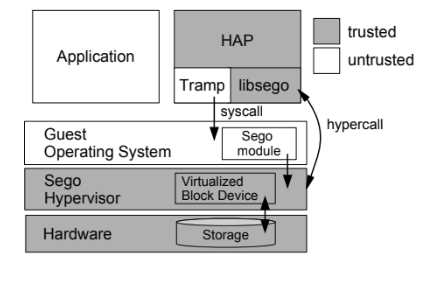
\includegraphics[width=0.5\linewidth]{sego_architecture}}%
	\caption{Sego Architecture Overview}
\end{figure}


Sego executes trusted code in a HAP. After booting the OS, the hypervisor starts the HAP in a way that the HAP itself can verify its own initial code and data, similar to a TPM. Once running, the hypervisor ensures that HAP's registers and trusted address space are isolated from the OS. 
Everytime the HAP wants to perform a system call, it must inform the hypervisor of its intent, so that the hypervisor can verify OS activity. HAPs use a small library called libsego as a way to handle system calls and get Sego services without having to change their code. 
Each HAP also contains an untrusted trampoline code, that uses to interact with the OS. This is used as a way to protect HAP control-flow, since it uses this trampoline as the issuer for the system calls, therefore never compromising the HAP itself. Figure 2.1 shows well enough Sego's overall design without going into to much dept, refering which components are included in the TCB and which are not. 

Context switches are handled by the hypervisor, hiding any information about the HAP from the OS.

Sego does not guarantee OS availability. A compromised OS can simply shut down or refuse to schedule processes. However this is easily detected.




\subsection{Other approaches}

There are also other approaches that tackle the same problem of trusting the OS, making it impossible for the execution of an  application to be compromised by a malicious OS, such as 

\begin{itemize}
	\item Hardware-assisted Data-Flow Isolation (HDFI) \cite{hdmiPaper} - data isolation mechanism running on top of RISC-V that uses machine instructions and hardware to enforce isolation, by virtually extending each memory unit with an additional tag that is defined by data-flow. It grants stack protection, standard library enhancement, kernel data protection, virtual function table protection, code pointer protection and information leak prevention. It's easy to use and imposes low performance overhead, while improving security.
	
	\item Secure Channel between Rich Execution Environment and Trusted Execution Environment (SeCReT) \cite{secretPaper} - it is a framework that is focused in securing the communications between the Rich Execution Environments (REE) and the TEE built in ARM TrustZone, to add to the idea of isolation from the OS. It enables legitimate processes to use a session key in the REE, which is regarded as unsafe. To protect the key, SeCReT verifies the code's integrity and control-flow of the process every time a switch between user mode and kernel mode takes place. SeCReT's key-protection mechanism is only activated during the runtime of the process that has permission to access TrustZone, so it minimizes the performance overhead.
	
	
\end{itemize}



\subsection{Discussion}

Another conclusion about the differences of the approaches. 
 
//TODO

Protection against untrusted OSes.

Virtual Ghost [20] uses both compile-time and run-time
monitoring to protect an application from a potentially-
compromised OS, but requires recompilation of the
guest OS and application.

Flicker [40], MUSHI [56],
SeCage [37], InkTag [21], and Sego [32] protect appli-
cations from untrusted OS using SMM mode or virtual-
ization to enforce memory isolation between the OS and
a trusted application.

Trustlite, isolate software
on low-cost embedded devices using a Memory Protec-
tion Unit.

Minibox built a 2-way sandbox for x86
by separating the Native Client (NaCl) [55] sandbox into
modules for sandboxing and service runtime to support
application execution and use Trustvisor [39] to protect
the piece of application logic from the untrusted OS.

Secret builds a secure channel to authenticate the appli-
cation in the Untrusted area isolated by the ARM Trust-
Zone technology.

HDFI extend each memory
unit with an additional tag to enforce fine-grained isola-
tion at machine word granularity in the HDFI system.







% section folder_structure (end)

% ===================
% = Package options =
% ===================
\section{SGX-Frameworks and Application Support} % (fold)
\label{sec:package_options}


The need for cloud computing is constantly growing in modern applications. It is a cost-effective and pratical solution to run large distributed applications, however the fact that it requires users to trust the cloud provider with their code and data creates some trust concerns for developers.
Although the usage of TEEs aim to tackle this problem by running and storing sensitive data on a isolated environment, protecting that data from unauthorized access. To accomplish this, the main approach is to devide the application into trusted and untrusted parts, reducing the TCB as much as possible as a way to reduce security breaches. 
In the next sections we'll discuss frameworks that can accomplish solutions to the problem described above, by working with Intel-SGX as the TEE provider, as a way to complement its regular execution.




\subsection{VC3 protection for MapReduce Jobs}

Verifiable Confidential Cloud Computing (VC3) \cite{vc3Paper} is a framework that achieves confidentiality and integrity of data, as well as verifiability of execution of code with good performance through MapReduce \cite{mapReduce} techniques. It uses Intel SGX processors as a building block and runs on unmodified Hadoop \cite{hadoop}.
In VC3 users implement MapReduce jobs, compile and encrypt them, thus obtaining a private enclave code E-. They then join it with a small portion of public code E+, that implements the protocols for key exchange and job execution.
Users then upload the resulting binary code to the cloud, where enclaves containing both E- and E+ are initialized by an untrusted framework F. 

\begin{figure}[htbp]
	\centering
	{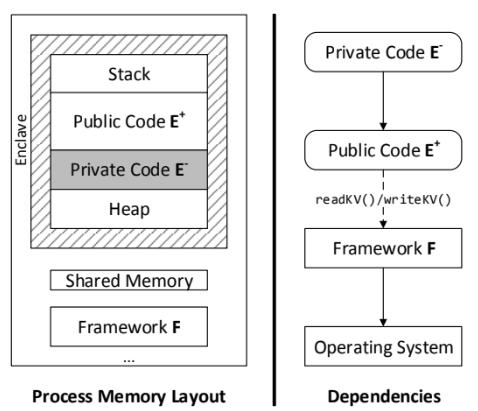
\includegraphics[width=0.6\linewidth]{vc3_design}}%
	\caption{VC3 memory design model on the left, component dependencies on the right}
\end{figure}

A MapReduce begins with a key exchange between the user and the E+ code running in the enclave. After this, E+ can proceed to decrypt E- and process the encrypted data. VC3 isolates this processing from the OS by keeping an interface between the E+ layer and the outside of the enclave. This interface consists of basically two functions: readKV() and writeKV(), for reading a key-value pair on Hadoop or write it, respectively. Also, the data inside of the enclave is passed to the outside, more specifically from E+ to the untrusted F, by using a virtual address space shared by both.
With VC3, both E- and the user data are always encrypted while in the cloud, except when processed by the trusted processor, while allowing Hadoop to manage the execution of VC3 jobs. Map and reduce nodes are seen as regular worker node to Hadoop, therefore Hadoop can provide its normal scheduling and fault-tolerance mechanisms, as well as load balancing. VC3 accomplishes this keeping Hadoop, the OS and the hypervisor out of the TCB.




\subsection{Protected ZooKeeper}

ZooKeeper \cite{zookeeper} is a replicated synchronization service for distributed systems with eventual consistency. However, ZooKeeper does not guarantee privacy of data stored inside of it by default.
 
Protected ZooKeeper \cite{protectedZooKeeper} is an approach that eliminates this privacy concerns, by placing an aditional layer between the client and the ZooKeeper, refered as ZooKeeper Privacy Proxy (ZPP). ZPP is a layer responsible for the encryption of all sensitive information, during a communication between a client and the ZooKeeper. 
Clients communicate with the proxy via a SSL connection, where the packets are encrypted by an individual session key. Here, ZPP acts like a normal ZooKeeper replica to the client. 
After receiving the packets from the client, ZPP extracts the sensitive data, encrypts it with a mechanism that allows the data to be decrypted by the proxy later on, and forwards the encrypted packet to a ZooKeeper replica where it can be stored with integrity ensured.
 
ZPP runs inside a TEE, located in the cloud, allowing it to store encryption keys and process plaintext data safely. As a result, even if the attacker is the cloud provider itself, the integrity of the data will still be granted since the attacker won't be able to access or alter anything running inside the TEE.

ZPP also retains all original ZooKeeper functionality, and does not affect ZooKeeper's internal behaviour. Therefore adapting existing ZooKeeper applications to this concept of ZPP it's easily done.

This approach allows applications in the cloud to use ZooKeeper without privacy concerns at the cost of a small decrease of throughput.

\subsection{Ryoan Sandboxing}

Ryoan \cite{ryoanPaper} consists on a distributed sandbox that allows users to protect the execution of their data. This is achieved with the help of Intel SGX \cite{intelSGX} \cite{sgxPaper} enclaves, creating sandbox instances that protect data from untrusted software while also preventing leaks of data, which is a weakness of enclaves caused by side channel attacks.
Ryoan does not include any priviledged software (e.g. OS and hypervisor) in it's TCB, while trusting only the hardware (SGX enclave) to assure secrecy and integrity of the data.

It's main goal is to prevent leakage of secret data. This is done by preventing modules from sending sensitive data over their communications if outside the system boundaries, as well as eliminating stores to unprotected memory and system calls, made possible by the use of a trusted sandbox Native Client (NaCl). 

\begin{figure}[htbp]
	\centering
	{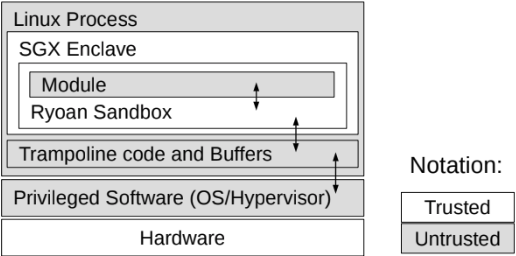
\includegraphics[width=0.6\linewidth]{ryoan_design}}%
	\caption{Instance of Ryoan running on a single machine}
\end{figure}

Ryoan's approach consists on confining the untrusted application in a NaCl, responsable of controlling system calls, I/O channels and data sizes. This NaCl sandbox is implemented inside the enclave, and can communicate with other instances of the NaCl, forming a distributed sandbox between users and different service providers. Inside the sandbox, the untrusted application can execute safely on secret data. The NaCl sandbox uses a load time code to ensure that the module can not do anything it shouldn't, thus violating the sandbox. To handle faults, exceptions or errors inside the NaCl sandbox, Ryoan uses an unprotected trampoline code, that can enter the enclave and read the information about the fault so it can handle it.



\subsection{Opaque}

Opaque \cite{opaquePaper} is a distributed data analytics platform that guarantee encryption, secure computation and integrity to a wide range of queries. Therefore, instead of being implemented in the application layer or the execution layer as this kind of security approaches usually are, Opaque is implemented in the query optimization layer. 

It is implemented with minimal modifications on Spark SQL, and uses Intel SGX technology as a way to grant confidentiality and integrity of the data. 
However, the use of enclaves can still be threatened by access pattern leakage that can occur at memory-level, when a malicious OS infers information about encrypted data just by monitoring memory page accesses, and at network-level, when network traffic reveals information about encrypted data.

Opaque hides access patterns in the system by using distributed oblivious relational operators and optimizes these by implementing new query planning techniques. It can be executed in three modes

\begin{itemize}
	\item encryption mode: provides data encryption and authentication, while granting correct execution.
	\item oblivious mode: provides oblivious execution, protecting against access pattern leakage.
	\item oblivious pad mode: extends the oblivious mode by adding prevention of size leakage.
\end{itemize}

Opaque is an approach that is able to grant oblivious execution 3 times faster than other specialized oblivious protocols.



\subsection{Graphene-SGX}

The usage of Intel SGX, and similar technologies, have proven to add a great sense of privacy to the storage and execution of data in applications. However this tecnologies impose restrictions (e.g., disallowing system calls inside the enclave) that require the applications to be changed so they can benefit from this extra layer of security. 

Graphene-SGX \cite{graphenePaper} came to help circunvent those restrictions, while still assure security to the data. It is a library OS that aims to reproduce system calls, respecting security concerns, so that unmodified applications can use them to keep executing normally without interacting directly with the OS or hypervisor. 

By using a library OS, the system is expected to lose performance and, since a new layer of software was added, to increase the size of the TCB. 
Although these assumptions are true, they are quite often exagerated. Graphene-SGX's performance goes from matching a Linux process to less than 2x in most executions of single-processes.
Graphene-SGX has also shown some great results comparing it to other similar approaches that use shim layers, such as SCONE \cite{sconePaper} and Panoply \cite{panoplyPaper}, where it shows to be performancewise similar to SCONE and faster 5-10 percent than Panoply, while adding 54k lines of code to the TCB compairing to SCONE's 97k and Panoply 20k.

Graphene's main goal is to run unmodified applications on SGX quickly. Thus, whilst the size of the TCB is not the smallest compairing to the other approaches, developers can reduce the TCB as needed as a way to reach a more optimal solution. 

Graphene-SGX also supports application partitioning, enabling it to run small pieces of one application in multiple enclaves. This can be useful, for instance, to applications with different privilege levels while still increasing the security of the application.

\subsection{Network services protection approaches}

Security and privacy have become one of the main concerns for both users and developers, therefore software technologies, like TLS and even anonymous networks like Tor, have become quite popular. At the same time, hardware approaches capable of providing TEEs (e.g. Intel-SGX) have also made contributions to help with this concerns. 
As these technologies are being adapted by applications, it's also believed that they can have a significant impact on networking, since it can be used, for instance, to solve policy privacy issues in inter-domain routing, thus protecting ISPs policies. 

In \cite{torSGXPaper}, it's shown that leveraging hardware protection of TEEs can grant benefits, such as simplify the overall design of the application, as well as securely introduce in-network functionality into TLS sessions. 
The same paper also presents a possible approach to reach security and privacy on a network level, by building a prototype on top of OpenSGX, that shows that SGX-enabled applications have modest performance losses compared to one with no SGX support, while significantly improving it's security and privacy.


-------

Network Function Virtualization (NFV) applications are stateful.
For example, a Content Distribution Network (CDN) caches web
contents from remote servers and serves them to clients. Similarly,
an Intrusion Detection System (IDS) and an Intrusion Prevention
System (IPS) have both per-flow and multi-flow (shared) states to
properly react to intrusions. On today’s NFV infrastructures, security vulnerabilities many allow attackers to steal and manipulate the
internal states of NFV applications that share a physical resource.
In this paper, we propose a new protection scheme, S-NFV that incorporates Intel Software Guard Extensions (Intel SGX) to securely
isolate the states of NFV applications.




-> S-NFV, provides a secure framework for NFV ap-
plications. S-NFV provides an interface to move the VNF states and
state processing code inside the enclave.
the framework needs to provide
a model to only allow relevant states (which need protection) to be
moved to the enclave. Also, for the framework to provide the right
abstraction for the different types of states (per-flow, shared, and
global), the challenge lies in understanding the state usage model
in various NFV applications. Along with securing VNF states, we
also propose secured administrator access to configure rules used by
these states and to view logs generated by these state processing.

RESULTS: In this paper, we took a first step toward protecting the internal
states of NFV applications against malicious hosts and buggy ap-
plications. By leveraging Intel SGX’s isolation, we demonstrated
the state protection of Snort’s internal state (TagNode) and its state
processing, by moving them into an enclave. We also perform the
preliminary evaluation on state processing operations using real
SGX hardware.



\subsection{Application-level protection approaches}

\subsection{Discussion}

Haven [15] showed
that a library OS could run unmodified applications on
SGX,

thin “shim” layers, like SCONE [14] and Panoply [49] wrap 
an API layer such as the system call table.


--------


SGX frameworks and applications.

VC3 [45]
runs MapReduce jobs in SGX enclaves.

Bren-
ner et al. [17] run cluster services in ZooKeeper in an
enclave, and transparently encrypt data in transit be-
tween enclaves.

Ryoan [22] sandboxes a piece of un-
trusted code in the enclave to process secret data while
preventing the loaded code from leaking secret data.

Opaque [57] uses an SGX-protected layer on the Spark
framework to generate oblivious relational operators that
hide the access patterns of distributed queries.

The \novathesis\ class can be customized with the options listed below.



\section{Related work analysis and rational} % (fold)
\label{sec:additional_considerations}

In this section we will provide some additional considerations about some of the customizations available as class options.



